\documentclass[times,10pt,twocolumn]{article} 
\usepackage{main}
\usepackage{times}
\usepackage[english]{babel}
\usepackage{hyperref}
\usepackage{listings}
\usepackage[utf8]{inputenc}
\usepackage{latexsym}
\usepackage{graphicx}
\pagestyle{empty}

\parindent0em

\begin{document}
\title{
LANA stack agreement protocol\\\smallskip [DRAFT]
}

\author{
Daniel Borkmann\\
dborkma@tik.ee.ethz.ch\\
}

\maketitle
\thispagestyle{empty}

\begin{abstract}
This report describes the LANA stack agreement protocol (LSAP). LSAP 
provides a definition for two communication endpoints on how they should 
symmetrically initiate their stack of functional blocks and how information
dispatch points (IDPs) for accessing respectivly addressing each others
entry point of the stack are exchanged. LSAP is a mandatory part of the 
basic LANA framework.
\end{abstract}

\Section{Introduction}
The LANA stack agreement protocol is necessary since communication partners can have 
a different set of functional blocks within their stack repository. In order 
to allow communication, it is needed to agree on a specific subset of 
functional blocks and on a specific binding of functional blocks of this 
subset, so that both ends have a symmetric structure of their communication
stacks.\newline

In the broad sense, this is similar to the Session Description Protocol (SDP)
\cite{VanJacobsonet.al.2006} of SIP \cite{HenningSchulzrinneet.al.2002} where
multimedia sessions as voice-over-IP calls are initiated and streaming
protocols or used codecs are negotiated.\newline

\textit{LSAP} itself does not incorporate a transport protocol and is intended 
to be used on different transport protocols as appropriate (really? See \ref{iss}). Its only purpose
is to describe the negotiation of used functional blocks in LANA for both 
communication partners, so that afterwards a communication on a certain
agreed protocol stack can be made possible.\newline

\Section{Functional Block Namespaces}
\label{fbns}
The functional block namespace must be independant of global, statically
assigned identifiers, so that the need for a central authority that maintains
such numbers will superfluous. For this purpose we orientate on module or 
package namespaces in programming languages where companies or single 
developers provide library code with a unique string identifier as a reference
where a certain method or function should be looked up and linked to the
application.\newline

Hence, we introduce namespaces for functional blocks in LANA, for having a 
specified dynamically assigned reference to functional blocks. We therefore 
define
\begin{quote}\texttt{namespace}\end{quote}
as an instance of a qualified functional block type of form \texttt{entity.id}
where \texttt{.} (dot) is a terminal symbol and both, \texttt{entity} and
\texttt{id} are meta symbols for \texttt{id} as an instance of 
$\mathcal{L}(id)=\{\alpha^{+}(\beta\alpha^{+})^{*}\} \;\vert\; \alpha\in\{a,b,c,\ldots,z,0,1,2,\ldots,9\},\beta\in\{$-$\}$
where elements of $\{a,b,c,\ldots,z,0,1,2,\ldots,9\}$ and $\{$-$\}$ are terminal symbols
and \texttt{entity}$\rightarrow$\texttt{id}$|$\texttt{entity.id}. With this
scheme, we have defined a qualified functional block type namespace in LANA.
Valid functional block type names are i.e.
\begin{itemize}
        \setlength{\itemsep}{-1mm}
	\item \texttt{ch.ethz.csg.dummy}
	\item \texttt{ch.ethz.csg.aes256}
\end{itemize}
However, an invalid example would be a functional block of type \texttt{dummy}
since this functional block type is not qualified.\newline

The semantic of the given valid example can be seen as: \texttt{ch.ethz.csg}
is a entity that provides a set of functional blocks for a given purpose, so
therefore \texttt{ch.ethz.csg} is a functional block provider. 
\texttt{ch.ethz.csg.aes256} in particular is a functional block type that
obviously provides \texttt{AES256} encryption provided by the \texttt{ch.ethz.csg}
entity.\newline

In the following we assume if two functional blocks are of type i.e. 
\texttt{ch.ethz.csg.aes256} then both functional blocks refer to one and the 
same underlying implementation. This also means, that for instance a functional
block of type \texttt{ch.ethz.csg.aes256} and a functional block of type
\texttt{ch.ethz.tik.aes256} are type-incompatible to each other and hence not
usable within one defined layer for building the functional block protocol stack.

\Section{Protocol Description}
Since the notion of functional block type namespaces has been defined, this
section can now focus on the design of the LANA stack agreement protocol.\newline

The LANA stack agreement protocol needs to be a four-way handshake protocol
initialed by the sender of a message i.e. via the first \texttt{sendto(2)}
system call. By handing a set of \texttt{communication flags} to the kernel, the
application defines its communication needs (features such as \textit{reliable},
\textit{confidential}, ...) to the kernel, thus a kernelspace LANA controller
composes one or more appropriate sets of functional blocks with concrete 
bindings. The resulting composition is named $X$.\newline

Now $X$ is given to the remote communication partner which chooses $x\in{}X$,
thus both then will use one concrete element out of the composition. IDPs to
the entry points to $x$ must also be provided to each communication partner 
$A$ and $B$, so that the handshake looks like:

\begin{enumerate}
        \setlength{\itemsep}{-1mm}
	\item \texttt{offer} from $A$ to $B$: $A$ sends $X$
	\item \texttt{select} from $B$ to $A$: $B$ selects $x\in{}X$, builds
              its stack according to $x$ and sends $x$ back to $A$ together 
              with its entry information dispatch point $IDP_B$ for the created
              communication stack
        \item \texttt{ack-1} from $A$ to $B$: $A$ acknowledges $IDP_B$
              to $B$, builds its stack according to $x$ and sends its entry
              information dispatch point $IDP_A$ for the created 
              communication stack
	\item \texttt{ack-2} from $B$ to $A$: $B$ acknowledges $IDP_A$
              to $A$
\end{enumerate}

Since the underlying carrier does not need to have an error-detecting code, each
message must have an error-detection i.e. a cyclic redundancy check. Also, since
communication can interrupt on both ends, timeouts must be provided to the
individual states, so that in case of an error respectively timeout, the 
created stack is being destroyed again or messages are being retransmitted.\newline

If the handshake has been done successfully the remotes IDP information is 
locally cached and associated to the socket until the socket is closed by the
application. A close will then implicitly incorporate a notification to the
opposite end, so that the remote stack is being destroyed, too:

\begin{enumerate}
        \setlength{\itemsep}{-1mm}
	\item \texttt{close} from $A$ to $B$: the $IDP_A$ is
              sent to the opposite end $B$ to notify that $B$s stack $x$
              that was previously built may now be released
	\item \texttt{ack-3} from $B$ to $A$: $B$ acknowledges the 
              reception of $IDP_A$ and sends $A$ its destroyed $IDP_B$
\end{enumerate}

\Section{Integration into LANA}
\begin{figure}[ht]
  \centering
  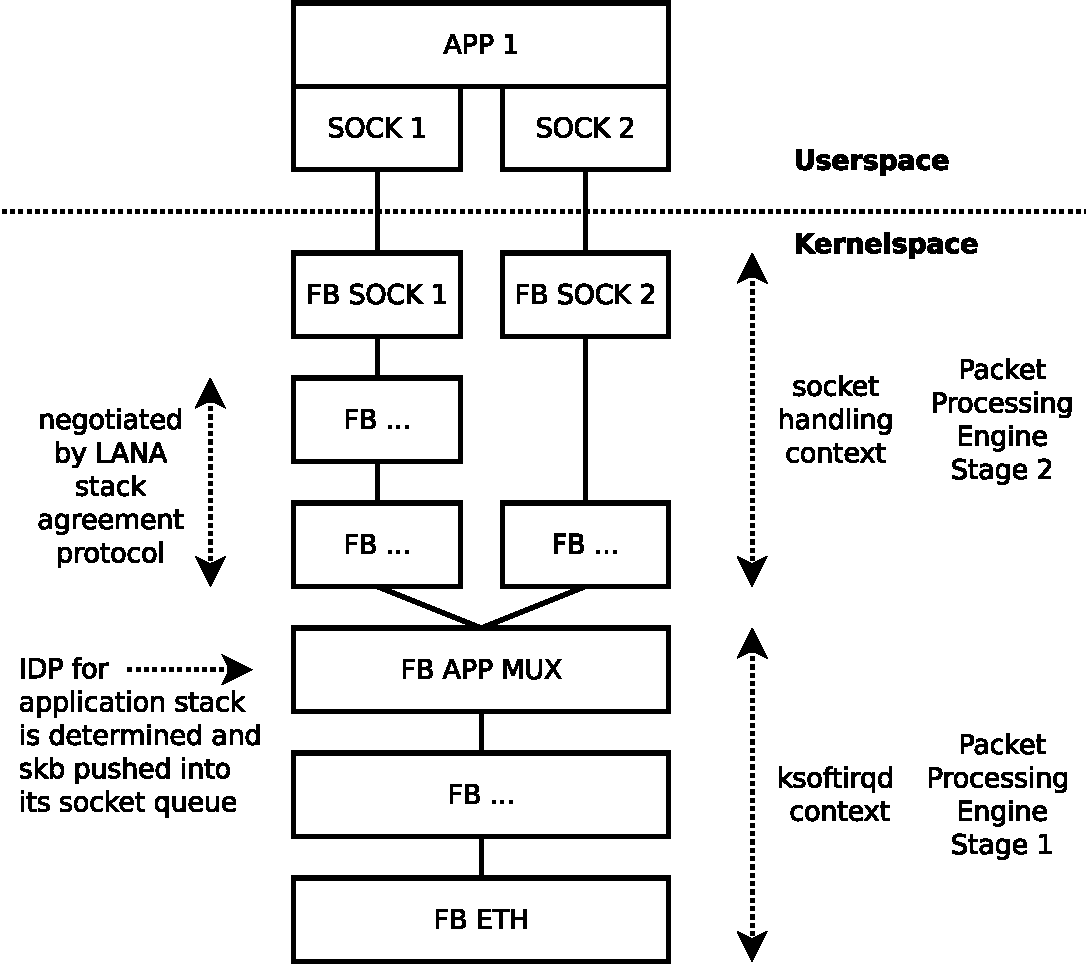
\includegraphics[width=0.5\textwidth]{stack.pdf}
  \caption{LANA functional block (FB) stack}
  \label{fig1}
\end{figure}

As shown in figure \ref{fig1}, LSAP is the protocol for building the 
application functional block stack that represents the glue between 
an underlying functional block structure for all packtes like traffic 
management functional blocks or packet filtering functional blocks 
up to the application multiplexing functional block and the userspace
application itself.\newline

There, a new socket is being registered at the \texttt{FB APP MUX}, so 
that incoming packets to this socket can be pushed into its socket queue
together with a next IDP information for a later processing within socket 
handling context. The \texttt{FB APP MUX} also keeps track of outgoing
packets, so that the next IDP information of the destination host is 
being added into the header field if the remote application stack has 
already been created.\newline

Offerings and selections during the stack agreement are outside of the 
context of \texttt{FB APP MUX}. Here, an external kernelspace LANA
controller (figure \ref{fig2}) is invoked for receiving the applications 
\texttt{communication flags} of \texttt{sendto(2)} and creating and 
appropriate stack offering message for the destination host. Therefore, 
the external controller knows of the whole local LANA functional block 
type repository.

\begin{figure}[ht]
  \centering
  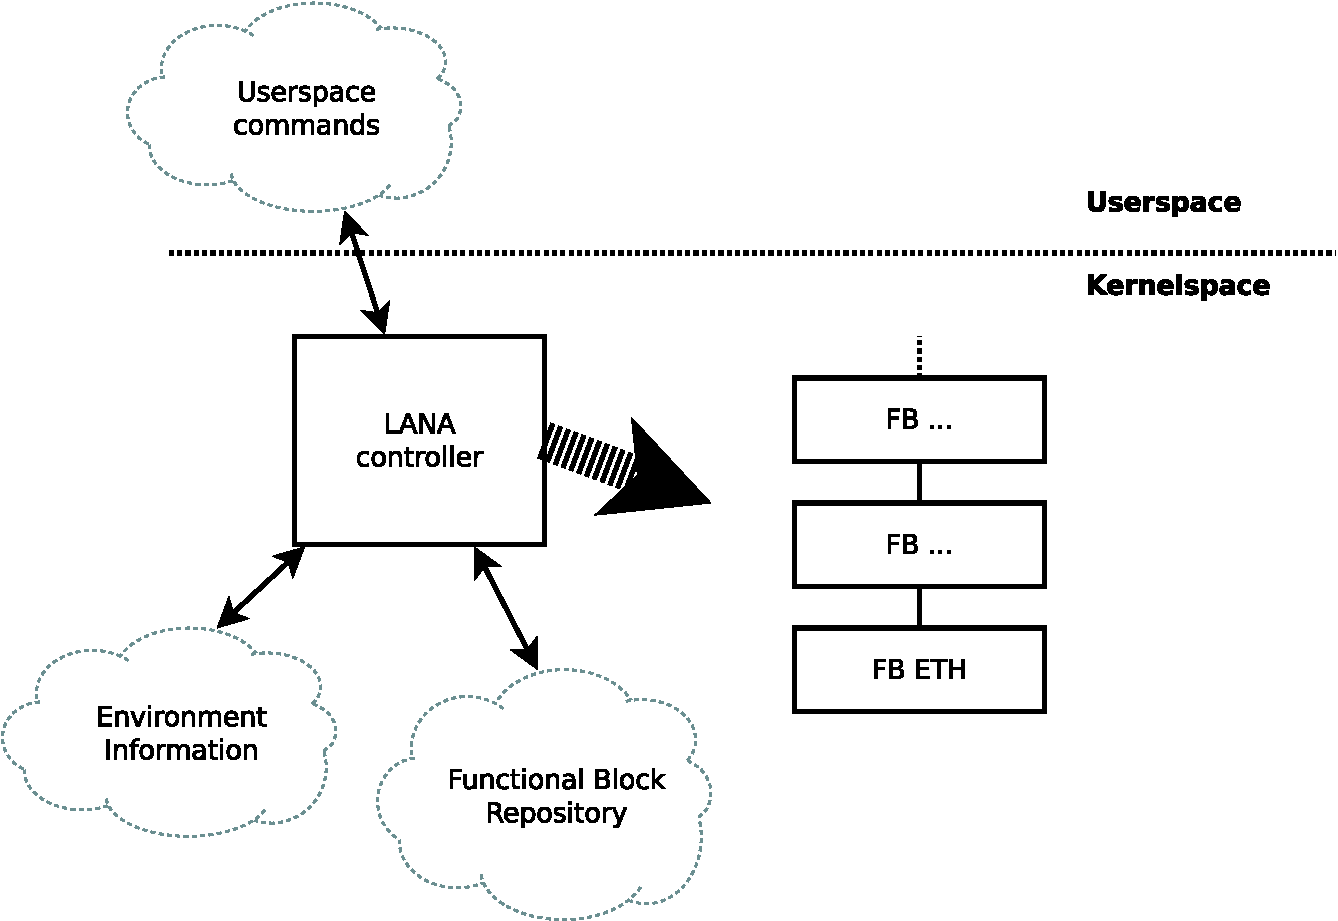
\includegraphics[width=0.5\textwidth]{controller.pdf}
  \caption{LANA controller}
  \label{fig2}
\end{figure}

\Section{Message Format}
The protocol header fields of LSAP are the following:
\begin{itemize}
        \setlength{\itemsep}{-1mm}
	\item \texttt{version, 3 Bit} protocol version major number
	\item \texttt{state, 5 Bit} current state
	\item \texttt{idp, 32 Bit} IDP number
	\item \texttt{ack, 32 Bit} Acked IDP number
	\item \texttt{happ, 20 Byte} Hash of socket application name
	\item \texttt{num, 8 Bit} Number of upcoming stack offerings
	\item \texttt{len, 16 Bit} Total length of stack offerings
	\item \texttt{crc, 32 Bit} Redundany check of stack offerings
	\item \texttt{stacks, variable} Stack offering payload
\end{itemize}

Format of \texttt{stacks}:
\begin{itemize}
        \setlength{\itemsep}{-1mm}
	\item \texttt{namespace} followed by \texttt{0x00}
	\item \texttt{namespace} followed by \texttt{0x00}
	\item \texttt{...}
	\item \texttt{namespace} followed by \texttt{0x11}
	\item \texttt{...}
	\item \texttt{namespace} followed by \texttt{0x00}
	\item \texttt{namespace} followed by \texttt{0x00}
	\item \texttt{...}
	\item \texttt{namespace} followed by \texttt{0x11}
\end{itemize}

The notion of \texttt{namespace} is defined in section \ref{fbns}.
The \texttt{0x00} character is meant as a separation symbol between
\texttt{namespace}s and the \texttt{0x11} character implies the end
of a stack description, so that multiple stacks can be described within
a single message. The order of \texttt{namespace}s within a stack 
description equals the binding order of functional block instances for
this description from lower to upper layers.\newline

A valid example of \texttt{stacks}:
\begin{itemize}
        \setlength{\itemsep}{-1mm}
	\item \texttt{ch.ethz.csg.dgram} + \texttt{0x00}
	\item \texttt{ch.ethz.csg.sip} + \texttt{0x00}
	\item \texttt{ch.ethz.csg.encryption} + \texttt{0x11}
	\item \texttt{ch.ethz.csg.dgram} + \texttt{0x00}
	\item \texttt{ch.ethz.tik.ssip} + \texttt{0x11}
\end{itemize}

This example demonstrates a description of two possible encrypted SIP stack
variants.

\Section{Example Handshake}
The following listing shows a complete example four-way LSAP handshake:
\scriptsize{
\begin{lstlisting}
A --> B:

version=1
state=1 (offer)
idp=24345 (random number)
ack=0
happ=7ecde348ff9cda2c3ba69a0c4543365039d0d65b
num=2
len=97
crc=<xyz>
stacks=
ch.ethz.csg.dgram + 0x00
ch.ethz.csg.sip + 0x00
ch.ethz.csg.encryption + 0x11
ch.ethz.csg.dgram + 0x00
ch.ethz.tik.ssip + 0x11

A <-- B:

version=1
state=2 (select)
idp=43523 (B's IDP)
ack=24345
happ=7ecde348ff9cda2c3ba69a0c4543365039d0d65b
num=1 (always 1)
len=60
crc=<xyz>
stacks=
ch.ethz.csg.dgram + 0x00
ch.ethz.csg.sip + 0x00
ch.ethz.csg.encryption + 0x11

A --> B:

version=1
state=3 (ack-1)
idp=34521 (A's IDP)
ack=43523 (B's IDP)
happ=7ecde348ff9cda2c3ba69a0c4543365039d0d65b
num=0
len=0
crc=0
stacks=

A <-- B:

version=1
state=4 (ack-2)
idp=43523 (B's IDP)
ack=34521 (A's IDP)
happ=7ecde348ff9cda2c3ba69a0c4543365039d0d65b
num=0
len=0
crc=0
stacks=
\end{lstlisting}
}
\normalsize

A \texttt{reset} directly after the \texttt{offer} during the handshake would
look like:
\scriptsize{
\begin{lstlisting}
A <-- B:

version=1
state=5 (reset)
idp=0
ack=24345
happ=7ecde348ff9cda2c3ba69a0c4543365039d0d65b
num=2
len=97
crc=<xyz>
stacks=
ch.ethz.csg.dgram + 0x00
ch.ethz.csg.sip + 0x00
ch.ethz.csg.encryption + 0x11
ch.ethz.csg.dgram + 0x00
ch.ethz.tik.ssip + 0x11
\end{lstlisting}
}
\normalsize

The next listing shows an example of a two-way LSAP close notification:
\scriptsize{
\begin{lstlisting}
A --> B:

version=1
state=6 (close)
idp=34521 (A's IDP to be closed)
ack=0
happ=7ecde348ff9cda2c3ba69a0c4543365039d0d65b
num=0
len=0
crc=0
stacks=

A <-- B:

version=1
state=7 (ack-3)
idp=43523 (B's IDP to be closed)
ack=34521 (A's IDP)
happ=7ecde348ff9cda2c3ba69a0c4543365039d0d65b
num=0
len=0
crc=0
stacks=
\end{lstlisting}
}
\normalsize

\Section{Open Issues or Facts to describe}
\label{iss}
\begin{itemize}
        \setlength{\itemsep}{-1mm}
	\item Chicken-and-egg problem: we want to describe a stack structure for
              communication, but then how to communicate the stack structure?!
	\item Stack is created from sender to receiver on first \texttt{sendto(2)}
	\item Can we somehow avoid the \texttt{happ}?
	\item If if two different applications want different stacks for one
	      socket, then we need another multiplexer before the \texttt{FB SOCKET}
	\item If if two different applications want same stacks for one
	      socket, then we use the same stack (needs ref counting) or create
	      another one?
	\item Should LSAP describe the \textit{whole} stack or only the 'application stack'?
	\item Should LSAP allow the description of options for functional blocks? (Rather not)
	\item PF\_LANA sockets must be a mandatory part of LANA, also the \texttt{APP MUX}?
	\item Should LSAP be independant of everything (except hardware address
	      layer) and come with routing, too?!
\end{itemize}

\Section{Security Issues}
\SubSection{LSAP fake-offer flooding}
An attacker $C$ could perform a denial of service attack on host $A$ or $B$ by
sending fake LANA \texttt{offer} messages, so that the opposite site builds 
application stacks and rans out of memory. This issue is similar to a TCP SYN 
flooding.\newline

Could be solved with a similar technique as SYN Cookies?!

\SubSection{LSAP fake-close}
An attacker $C$ could perform a brute-force attack over all possible IDP numbers, 
so that fake close messages are generated in the hope, that the attacked host $B$
has an IDP pair $IDP_A,IDP_B$ where $IDP_C$ equals $IDP_A$, thus the connection
from $A$ to $B$ is being closed.\newline

Could be solved with cryptographic Session Cookies?!

\nocite{*}
\bibliographystyle{abbrv}
\bibliography{main}

\end{document}
